\documentclass[handout,xcolor={usenames,dvipsnames},11pt]{beamer}

\defbeamertemplate{description item}{align left}{\insertdescriptionitem\hfill}

% \usetheme[sectionpage=none,subsectionpage=simple,progressbar=none,block=fill]{metropolis}
\usetheme[sectionpage=none,subsectionpage=simple,progressbar=frametitle,block=fill]{metropolis}
% \setsansfont[BoldFont={Fira Sans SemiBold}]{Fira Sans Book}
\usepackage{tikz}
\usetikzlibrary{patterns}
\usetikzlibrary{shapes.misc, positioning}
\usepackage{eso-pic}
\usepackage{booktabs}
\usepackage[scale=2]{ccicons}
\usepackage{pgfplots}
\usepackage{amsmath}
\usepackage{wasysym}
\usepackage{mathtools}
\usepackage{pgf}
\usepackage{pifont}
\usepackage{algpseudocode}
\usepackage{listings}
% \setsansfont{Ubuntu}
% \setmonofont{Ubuntu Mono}

\DeclarePairedDelimiter{\ceil}{\lceil}{\rceil}
\usepgfplotslibrary{dateplot}
\hypersetup{colorlinks,linkcolor=Cerulean,urlcolor=Cyan}

\usepackage{xspace}
\newcommand{\themename}{\textbf{\textsc{metropolis}}\xspace}
\usefonttheme[onlymath]{serif}
\setbeamertemplate{caption}{\raggedright\insertcaption\par}


\title{ \Large Turbo Codes for Deep Space Communications: CCSDS 131.0-B-2 standard implementation}
% \title{\LARGE Reccomendation for Space Data System Standards}
% \title{\Large Metropolis}
\subtitle{Final project for the Channel Coding course}
\author[G. Marcon]{Gianluca Marcon \hfill \href{mailto:gianluca.marcon.1@studenti.unipd.it}{gianluca.marcon.1@studenti.unipd.it}}
\date{\today}
\institute{University of Padova}
% \institute{Department of Information Engineering, University of Padova}

% logo on every page
%\newcommand{\nologo}{\setbeamertemplate{logo}{}}

%\newcommand\AtPagemyUpperLeft[1]{\AtPageLowerLeft{%
%\put(\LenToUnit{0.94\paperwidth},\LenToUnit{0.03\paperheight}){#1}}}
%\AddToShipoutPictureFG{
%  \AtPagemyUpperLeft{{
\includegraphics[height=2cm,keepaspectratio]{./logos/DEI.png}}}
%}%

\logo{\vspace*{-1.4cm}
\includegraphics[height=2cm,keepaspectratio]{./logos/DEI.png}}


% full logo on title page
\titlegraphic{
\includegraphics[height=2cm]{./logos/unipd}\hfill
\includegraphics[height=2cm]{./logos/DEI_full}}
\setbeamertemplate{subsection page}[simple]

\begin{document}

\maketitle

%======================================================================================
\section{Introduction}
\begin{frame}{Standard specifications}
    The standard specifies different input packet lengths $k$
    \begin{itemize}
        \item $1784$
        \item $3568$
        \item $7136$
        \item $8920$
    \end{itemize}\pause

    ...and different code rates $R$
    \begin{itemize}
        \item $1/2$
        \item $1/3$
        \item $1/4$
        \item $1/6$
    \end{itemize}    
\end{frame}
%======================================================================================
\begin{frame}{Encoder structure}
    \begin{figure}
        \centering
        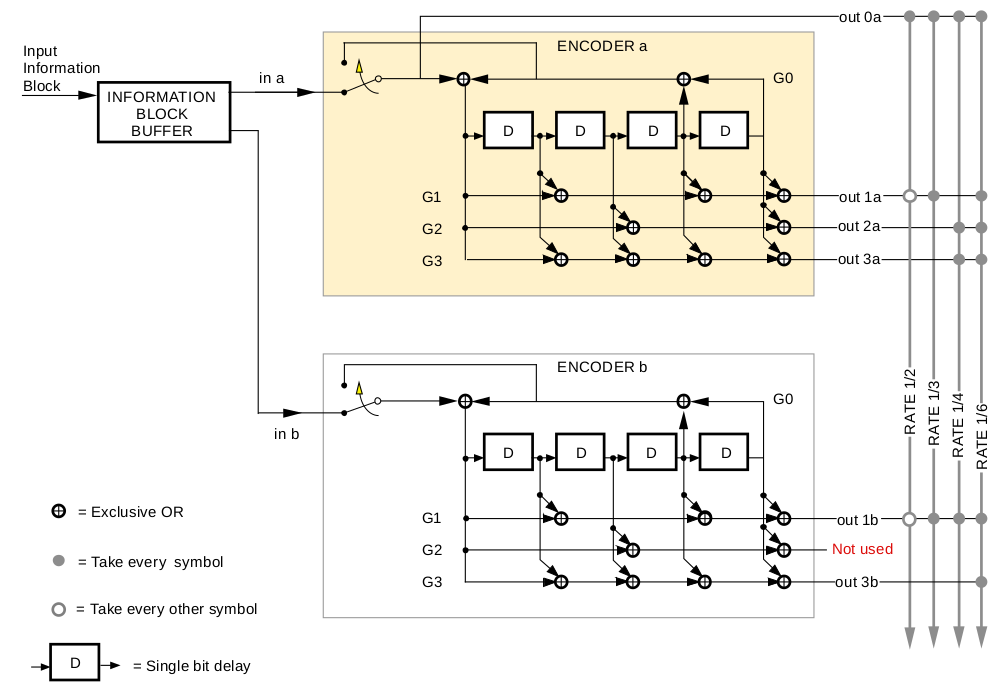
\includegraphics[height=0.75\textheight]{./images/encoder-structure}
    \end{figure}
    Convolutional codes defined through forward and backward connection vectors
\end{frame}

%======================================================================================
\begin{frame}[c,fragile]{Example: defining a code in C}
    \begin{lstlisting}[
        language=C,
        basicstyle=\scriptsize,
        commentstyle=\color{mLightGreen},
        stringstyle=\color{mLightRed}
        ]
    // define first code
    int N_components = 2;
    char *forward[N_components];
    forward[0] = "10011";
    forward[1] = "10101";

    char *backward = "0011";

    t_convcode code = convcode_initialize(forward, backward, 
                                            N_components);

    t_turbocode turbo = turbo_initialize(code, code, pi,
                                            info_length);
    \end{lstlisting}
    
\end{frame}
%======================================================================================
\begin{frame}{Interleaver}
    \begin{figure}
        \centering
        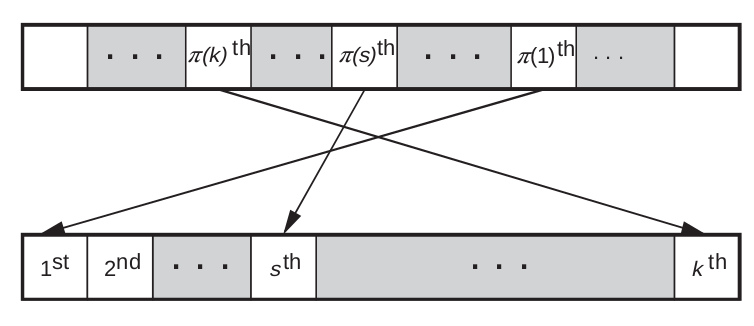
\includegraphics[width=0.5\textwidth]{./images/interleaver}
    \end{figure}
    
    $i$-th bit of the interleaved packet is the $\pi(i)$-th bit of the original packet

    \begin{table}
        \centering
        \begin{tabular}{ccc}
            \toprule
            Information block length & $k_1$ & $k_2$\\
            \midrule
                1784    &   8  &     223$\\
                3568    &   8  &     223$\times$ 2\\
                7136    &   8  &     223$\times$ 4\\
                8920    &   8  &     223$\times$ 5\\
            \bottomrule
        \end{tabular}
    \end{table}
\end{frame}

%======================================================================================
\begin{frame}{Building the interleaver}
    \begin{algorithmic}
        \State $p = \begin{bmatrix}31 & 37 & 43 & 47 & 53 & 59 & 61 & 67\end{bmatrix}$
        \For{$s = 1$ to $k$}
            \State $m = (s-1) \mod 2$
            \State $i = \text{floor}\left[(s-1)/(2k_2)\right]$
            \State $j = \text{floor}\left[(s-1)/2\right] -i k_2$
            \State $t = (19i + 1) \mod (k_1/2)$
            \State $q = t \mod 8 + 1$
            \State $c = (p_q j + 21m) \mod k_2$
            \State $\pi(s) = 2(t + c k_1/2 +1) - m$
        \EndFor
    \end{algorithmic}
\end{frame}

%======================================================================================
\begin{frame}[c]{Decoding}
    \begin{itemize}
        \item BCJR (in log domain) on upper and lower code
        \item scheduling as seen in class
        \item number of iterations is tuned accordingly
        \item puncturing is applied at reception for an easier implementation
            $\hat{r}[i] = r[i]\cdot p[i]$, $ 1 \leq i \leq (k+4)/R$
    \end{itemize}
    
\end{frame}
%======================================================================================
\begin{frame}[c,fragile]{Example: defining a code in C}
    \begin{lstlisting}[
        language=C,
        basicstyle=\scriptsize,
        commentstyle=\color{mLightGreen},
        stringstyle=\color{mLightRed}
        ]
        int *decoded = NULL;
        for (int i = 0; i < iterations; i++) {

            // run BCJR on upper code
            convcode_extrinsic(streams[0], lengths[0], 
                                 &messages, code.upper_code,
                                 noise_variance, 0);
            // apply interleaver
            message_interleave(&messages, code);

            // run BCJR on lower code
            decoded = convcode_extrinsic(streams[1], lengths[1], 
                                 &messages, code.lower_code, 
                                 noise_variance, 
                                 i == (iterations - 1));
            // deinterleave
            message_deinterleave(&messages, code);
        }
    \end{lstlisting}
\end{frame}

%======================================================================================
\begin{frame}[c]{Effect of increasing number of iterations}
    \begin{figure}
        \centering
       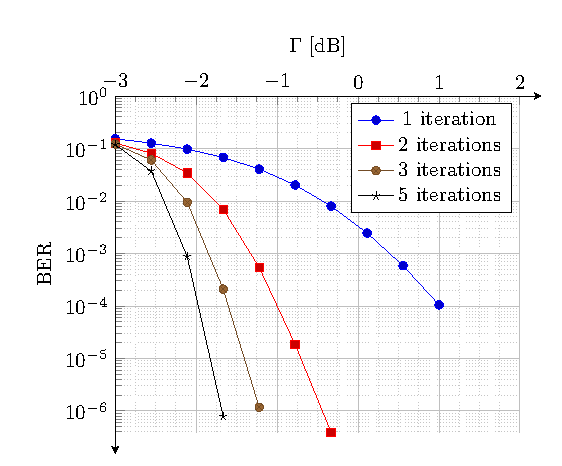
\includegraphics[height=0.9\textheight]{./images/BER}
    \end{figure}
\end{frame}
%======================================================================================
\begin{frame}[c]{Effect of increasing number of iterations}
    \begin{figure}
        \centering
       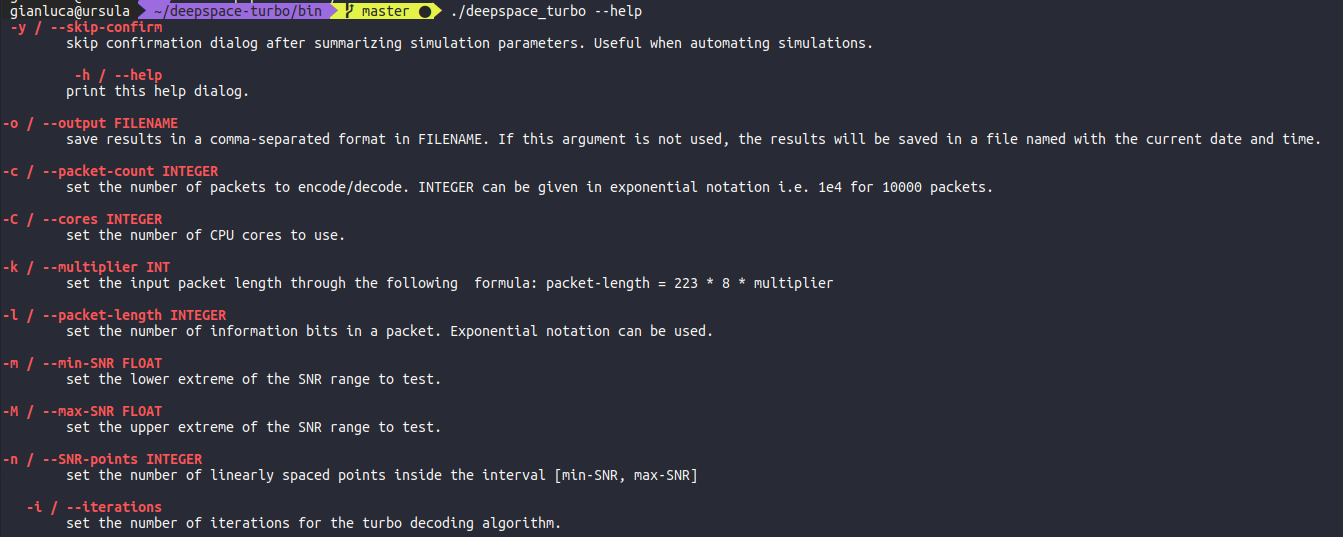
\includegraphics[width=1\textwidth]{./images/terminal}
    \end{figure}
\end{frame}
%======================================================================================
\begin{frame}[c]{Different packet sizes}
    
\end{frame}
%======================================================================================
\begin{frame}[c]{First type of modulator}
    \begin{figure}
        \begin{center}
           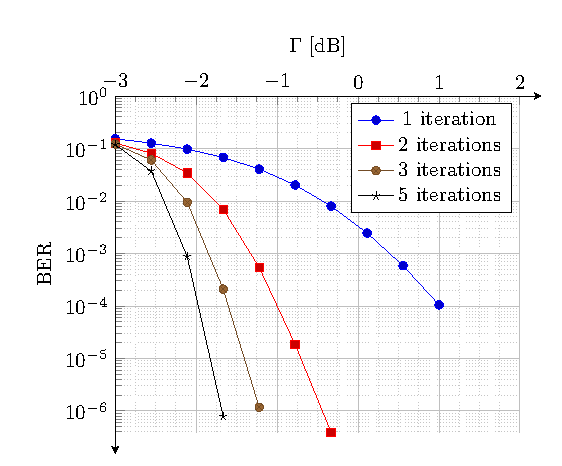
\includegraphics[width=0.6\textwidth]{./images/BER}
        \end{center}
        \caption{\cite{Cho2011}}
    \end{figure}\pause
    \begin{center}
        Large footprint required to obtain adequate modulation depth        
    \end{center}
\end{frame}
%======================================================================================
\begin{frame}[c]{Novel design: slot waveguides}
    \begin{figure}
        \centering
        \begin{tikzpicture}
            \node (img3) {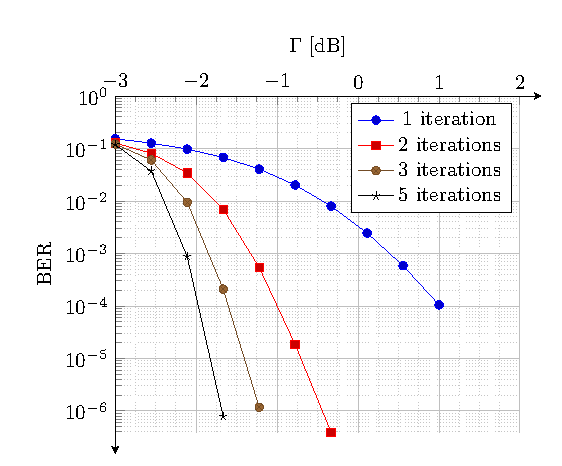
\includegraphics[height=3.5cm]{./images/BER}};
            \node (img4) at (img3.east)[xshift=2.5cm] {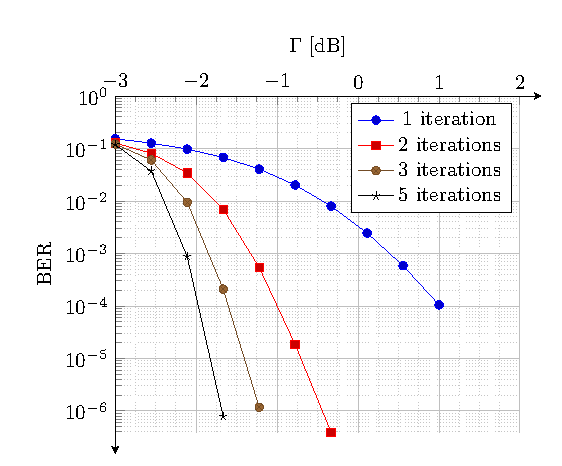
\includegraphics[height=3.5cm]{./images/BER}};
        \end{tikzpicture}
        \caption{$\lambda = 1550$ nm, $n_{co} = 1.46$, $n_{cl} = 3.48$, $w_{co} = 101$ nm. \cite{Xu2004}}
    \end{figure}\pause
    \begin{alertblock}{Absorbed power per unit area}
        \[
            P \propto \frac{1}{2} |\mathbf{E}| \cdot \frac{Im\{\varepsilon_{eff}\}}{|\varepsilon_{eff}|} 
        \]
    \end{alertblock}
\end{frame}  
%======================================================================================
\begin{frame}{Wavelength and Voltage dependency}
    \begin{figure}
        \centering
        \begin{tikzpicture}
            \node (img3) {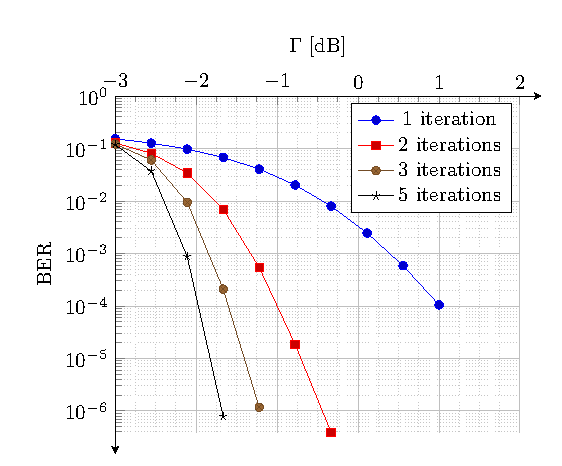
\includegraphics[height=4cm]{./images/BER}};
            \node (text1) at (img3.south)[yshift=-0.3cm]{Bandwidth > 1.25 THz};
            \node (img4) at (img3.east)[xshift=2.5cm] {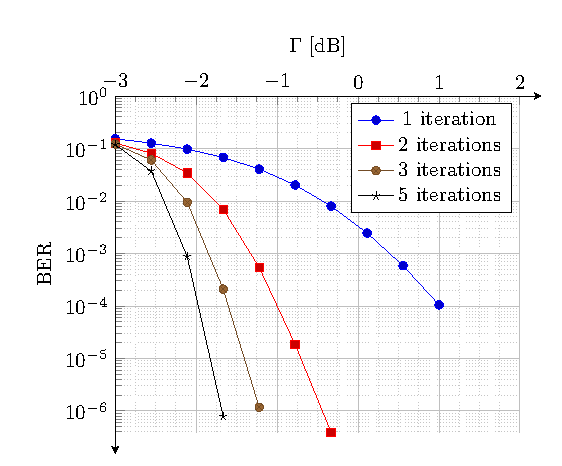
\includegraphics[height=4cm]{./images/BER}};
            \node (text2) at (img4.south)[yshift=-0.3cm]{$\Delta V = 1.32 V$};
        \end{tikzpicture}
    \end{figure}
    
\end{frame}
%======================================================================================
\begin{frame}[c]{Plasmonic-graphene waveguide modulator}
    \begin{figure}
        \centering
        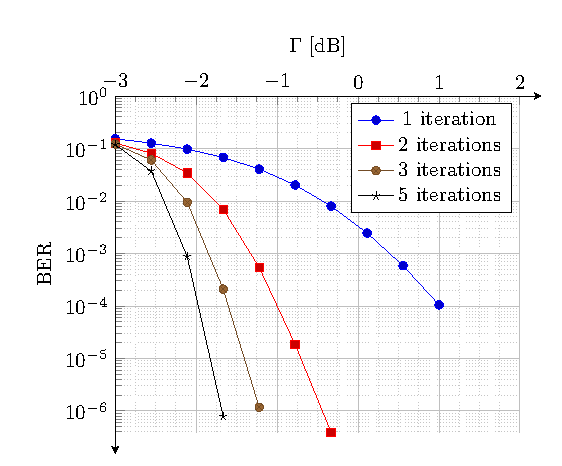
\includegraphics[height=4cm]{./images/BER}
    \end{figure}
    
    Cu is preferred (CMOS compatible), but has higher losses than Au, Ag.
\end{frame}
\begin{frame}{Plasmonic-graphene waveguide modulator}
    200 nm wide, silicone nitride 10 nm thick (both layers), length 120 nm.
    \begin{figure}
        \centering
        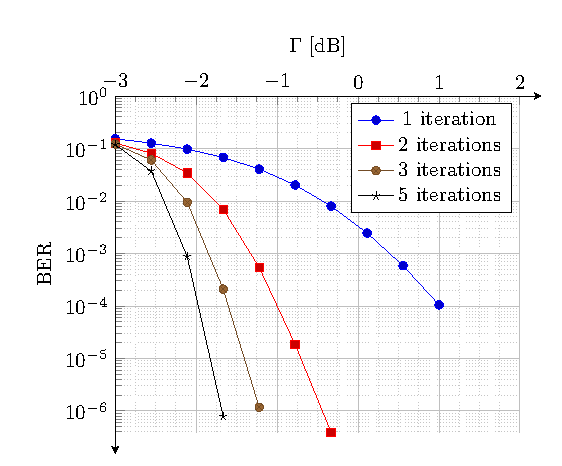
\includegraphics[width=0.5\textwidth]{./images/BER}
    \end{figure}    
    \begin{center}
        Footprint $ \sim 2-3 \;\mu m^2$
    \end{center}
\end{frame}
%======================================================================================
\begin{frame}{Wavelength and Voltage dependency}
    \begin{figure}
        \centering
        \begin{tikzpicture}
            \node (img3) {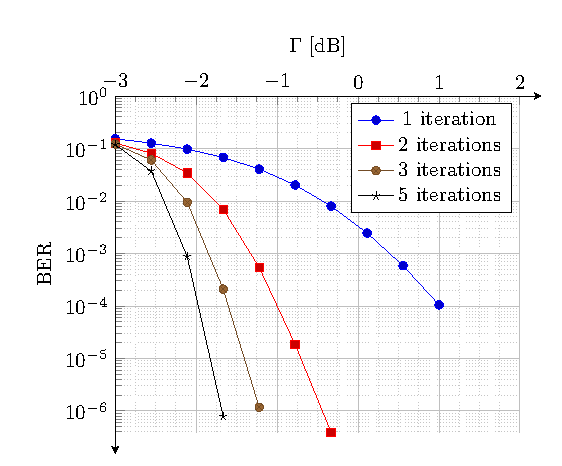
\includegraphics[height=4cm]{./images/BER}};
            \node (text1) at (img3.south)[yshift=-0.3cm]{Bandwidth > 1 THz};
            \node (img4) at (img3.east)[xshift=2.7cm] {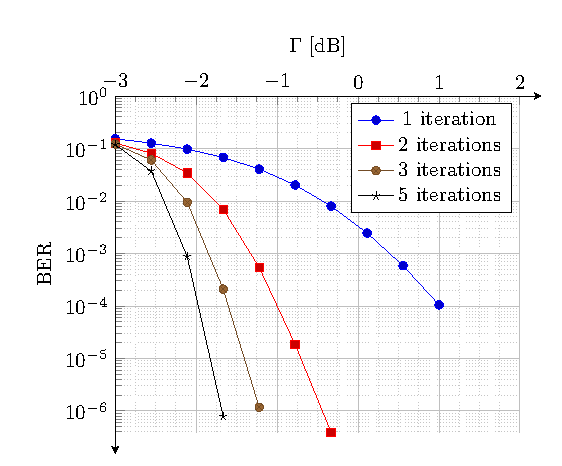
\includegraphics[height=4cm]{./images/BER}};
            \node (text2) at (img4.south)[yshift=-0.3cm]{$\Delta V = 1.38 V$};
        \end{tikzpicture}
    \end{figure}
    \begin{center}
        Energy consumption $\sim$ 0.12-0.13 pJ/bit
    \end{center}
\end{frame}
%======================================================================================
\begin{frame}{Did we meet any requirement?}
    \pause
    \begin{itemize}
        \item high bandwidth\pause\qquad \textcolor{TolLightGreen}{\textbf{Yes}}\pause
        \item energy efficiency\pause\qquad \textcolor{TolLightGreen}{\textbf{Yes}}\pause
    \item compatibility with on-chip electronic components\pause\quad \textcolor{TolLightGreen}{\textbf{Yes}}\pause
        \item low insertion loss\pause\qquad \textcolor{TolLightGreen}{\textbf{Yes}}\pause
        \item small footprint \pause\qquad \alert{\textbf{Kinda}} \pause
        \item high switching speed\pause\qquad \alert{\textbf{Potentially}}
    \end{itemize}
    % Usually can't meet every requirement. 
\end{frame}
%======================================================================================
\begin{frame}{Recent advances: graphene-on-silicon MZI}
    \begin{itemize}
        \item Fix one arm in "dielectric state" (low loss) of graphene
        \item Exploit changes in $Re\{ \varepsilon_{eff}\}$ wrt gate voltage to induce phase change
    \end{itemize}
    \begin{figure}
        \centering
        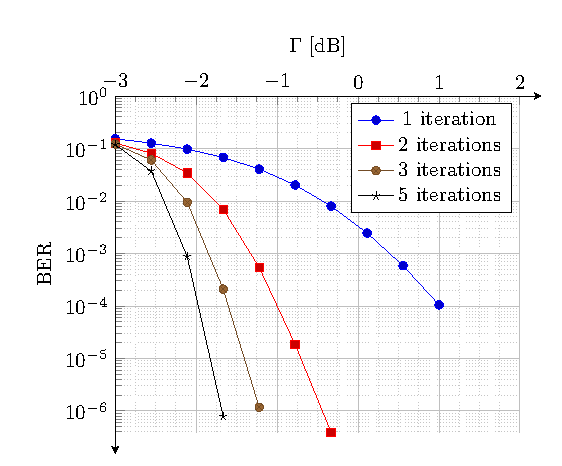
\includegraphics[width=0.5\textwidth]{./images/BER}
        \caption{\cite{Phatak2016}}
    \end{figure}
    %    Some references to showcase [allowframebreaks] \cite{knuth92,ConcreteMath,Simpson,Er01,greenwade93}
\end{frame}
%======================================================================================
\appendix

\begin{frame}[allowframebreaks]{References}
  \bibliography{presentation}
  \bibliographystyle{apalike}
\end{frame}

\begin{frame}[standout]
    Thank you!
\end{frame}
% %======================================================================================

\end{document}
